\begin{frame}{Introduction}
    \begin{columns}[T]
        \begin{column}{.6\textwidth}
            \textbf{What if?} Consider communication with an alien\ldots
            \begin{itemize}
                \item<1-> Before flying by we want to know: is alien world made out of \textbf{anti-matter}\ftnt{}?
                \item<1-> Can we propose an experiment to find out?
                \item<2> Where not to look for: QED, QCD (neither \textbf{C}harge (C), nor \textbf{P}arity (P), nor \textbf{T}ime reversal (T) symmetry is broken here
                \item<2> What about weak interaction?
                \begin{itemize}
                    \item<2> P violation measured with Wu-Experiment!
                    \item<2> \ldots but asymmetry cancels exactly when using anti-matter
                    \item<2> \textbf{Is definition of anti-matter ambiguous?}
                \end{itemize}
            \end{itemize}
        \end{column}
        \begin{column}{.4\textwidth}
            \centering
            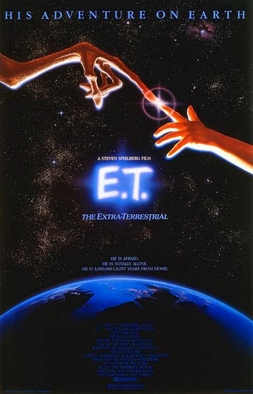
\includegraphics[height=.7\textheight]{et}\\
            {\tiny (Image: John Alvin, (c) 1982 Universal Studios)}
        \end{column}
    \end{columns}

    \vfill

    \footnotesize \ftnt{\cf{} fermions: if $\psi$ obeys $(\mathrm{i}\slashed\partial-m)\psi=0$, then $(\operatorname{CP}\psi)$ is also a solution (\textbf{C}harge and \textbf{P}arity inverted)}
\end{frame}

\begin{frame}{On the other hand\ldots}
    \begin{columns}[T]
        \begin{column}{.6\textwidth}
            \begin{itemize}
				\item Baryon asymmetry of the Universe:
                \begin{equation*}
                    \mathcal{O}(\eta_\text{cosm}) = \mathcal{O} \! \left( \frac{n_B - n_{\overline{B}}}{n_\gamma} \right) \sim 10^{-10} \neq 0,
                \end{equation*}
                with $n_{B,\overline{B},\gamma}=$ number of baryons, anti-baryons and photons
                \item Universe is filled with matter (rather than anti-matter\ftnt)
                \item Standard Model of Cosmology: Big Bang produces $n_B = n_{\overline{B}}$~~(\textbf{CP invariant})
                \item Evolution: QED and QCD are \textbf{CP invariant}
            \end{itemize}
        \end{column}
        \begin{column}{.4\textwidth}
        \end{column}
    \end{columns}

    \vspace{5mm}
    \footnotesize \ftnt{} \textit{i.e.}, most likely alien world is made out of matter as well
\end{frame}

\begin{frame}{Introduction}
    \begin{columns}[T]
        \begin{column}{.6\textwidth}
			\scalebox{1.2}{Can we explain $\mathcal{O}(\eta_\text{cosm})$?}
            \begin{itemize}
                \item \textbf{No!} We fail to describe one of the most obvious property of our Universe!
            \end{itemize}
            Can we (at least) describe some CP violating processes?
            \begin{itemize}
                \item Yes! The Standard Model of Particle Physics contains a CP violating sector (weak interaction)
                \item However, it does not predict the right order of magnitude of $\eta_\text{cosm}$\,!
            \end{itemize}
        \end{column}
        \begin{column}{.4\textwidth}
            \centering
            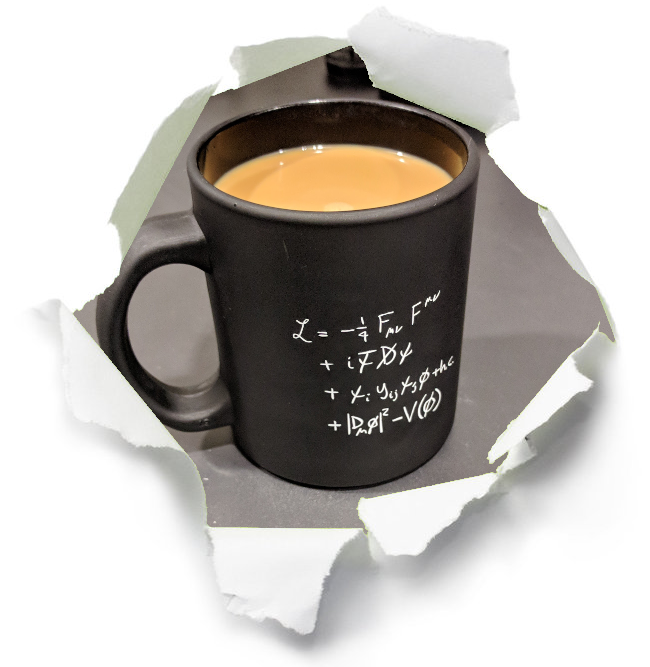
\includegraphics[height=.7\textheight]{cup}
        \end{column}
    \end{columns}
\end{frame}

\begin{frame}{Introduction}
    \begin{itemize}
        \item Diagonalizing Yukawa matrices\ftnt{} leads to \textbf{quark \textcolor{vertexDarkRed}{mass} eigenstates} $q$, but skews \textbf{quark \textcolor{vertexDarkRed}{flavor} eigenstates} $q'$
        \begin{equation*}
            \mathcal{J}^\mu_{\!cc} \; \supset \;
            (\overline{u'},\, \overline{c'},\, \overline{t'}) \, \gamma^\mu \frac{1-\gamma^5}{2} \begin{pmatrix}d' \\ s' \\ b' \end{pmatrix}
            \quad \longrightarrow \quad
            (\overline{u},\, \overline{c},\, \overline{t}) \, \gamma^\mu \frac{1-\gamma^5}{2} V_\text{\!CKM} \begin{pmatrix}d \\ s \\ b \end{pmatrix}
        \end{equation*}
        \begin{center}
            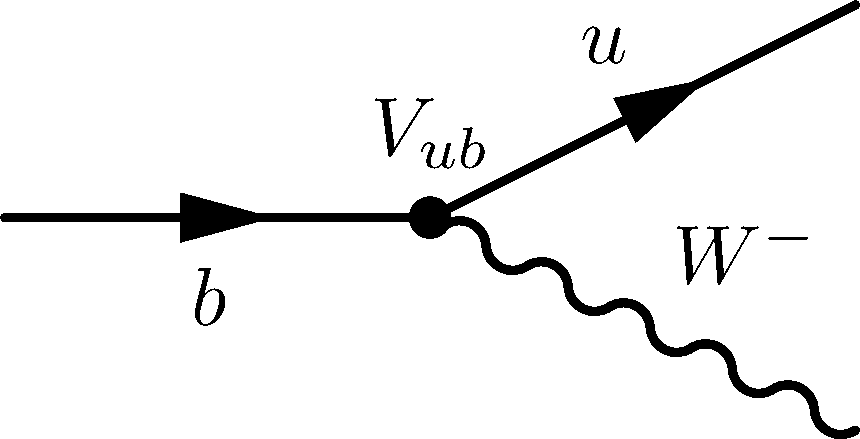
\includegraphics[width=.2\textwidth,valign=c]{decay_b2u}
            \scalebox{1.5}{\;+\;}
            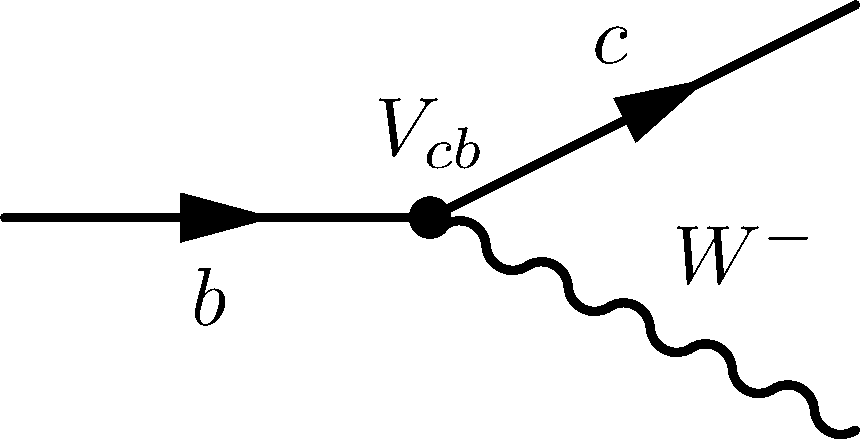
\includegraphics[width=.2\textwidth,valign=c]{decay_b2c}
            \scalebox{1.5}{\;+\;}
            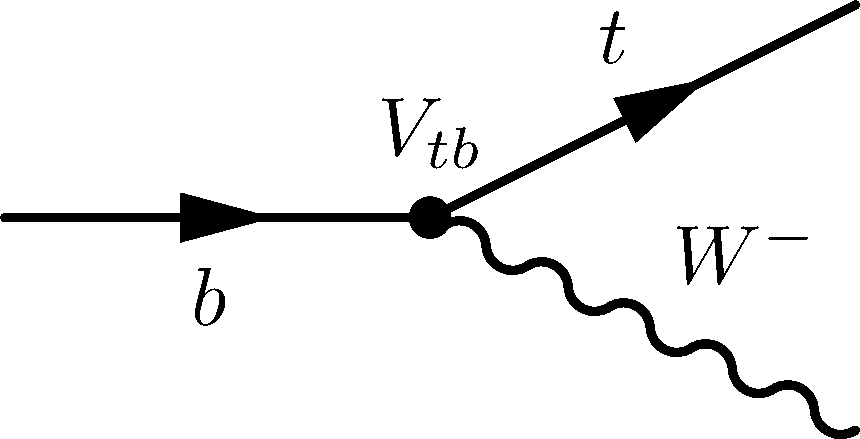
\includegraphics[width=.2\textwidth,valign=c]{decay_b2t}
        \end{center}
        \vspace{1em}
        \item This introduces the non-trivial transformation matrix $V_\text{CKM}$ for quarks (CKM matrix)
        \item $V_\text{CKM}$ is a \textbf{unitary} $3 \times 3$ matrix (CP violation \textit{in} complex phases)
    \end{itemize}

    \vspace{5mm}
    \footnotesize \ftnt{}\textit{cf.} Higgs mechanism
\end{frame}

\begin{frame}{State-of-the-art}
    \textbf{What we know}
    \begin{itemize}
        \item We understand CP violation (CPV) on quark level in the framework of the Standard Model (SM)
        \item CPV is predicted and confirmed with high confidence for \textbf{mesons}\ftnt{} at particle accelerators
    \end{itemize}
    \textbf{What we don't know}
    \begin{itemize}
        \item Absence of anti-\textbf{baryons}\ftnt{} is a large scale CPV which we cannot explain
        \item (strong CPV, neutrino CPV, Sakharov conditions, \ldots)
    \end{itemize}

    \textbf{Idea of this analysis}
    \begin{itemize}
        \item Establish (yet unknown) \textbf{baryon} decay which can be used (in the future) to measure CPV parameter of the SM
    \end{itemize}

    \vfill

    \footnotesize\ftnt meson / anti-meson: $(\quark\quarkbar)$, baryon: $(\quark\quark\quark)$, anti-baryon: $(\quarkbar\quarkbar\quarkbar)$
\end{frame}

\begin{frame}{The decay \decay{\Lb}{\Dz\Lz}}
    \begin{columns}[T]
        \begin{column}{.45\textwidth}
            \centering
            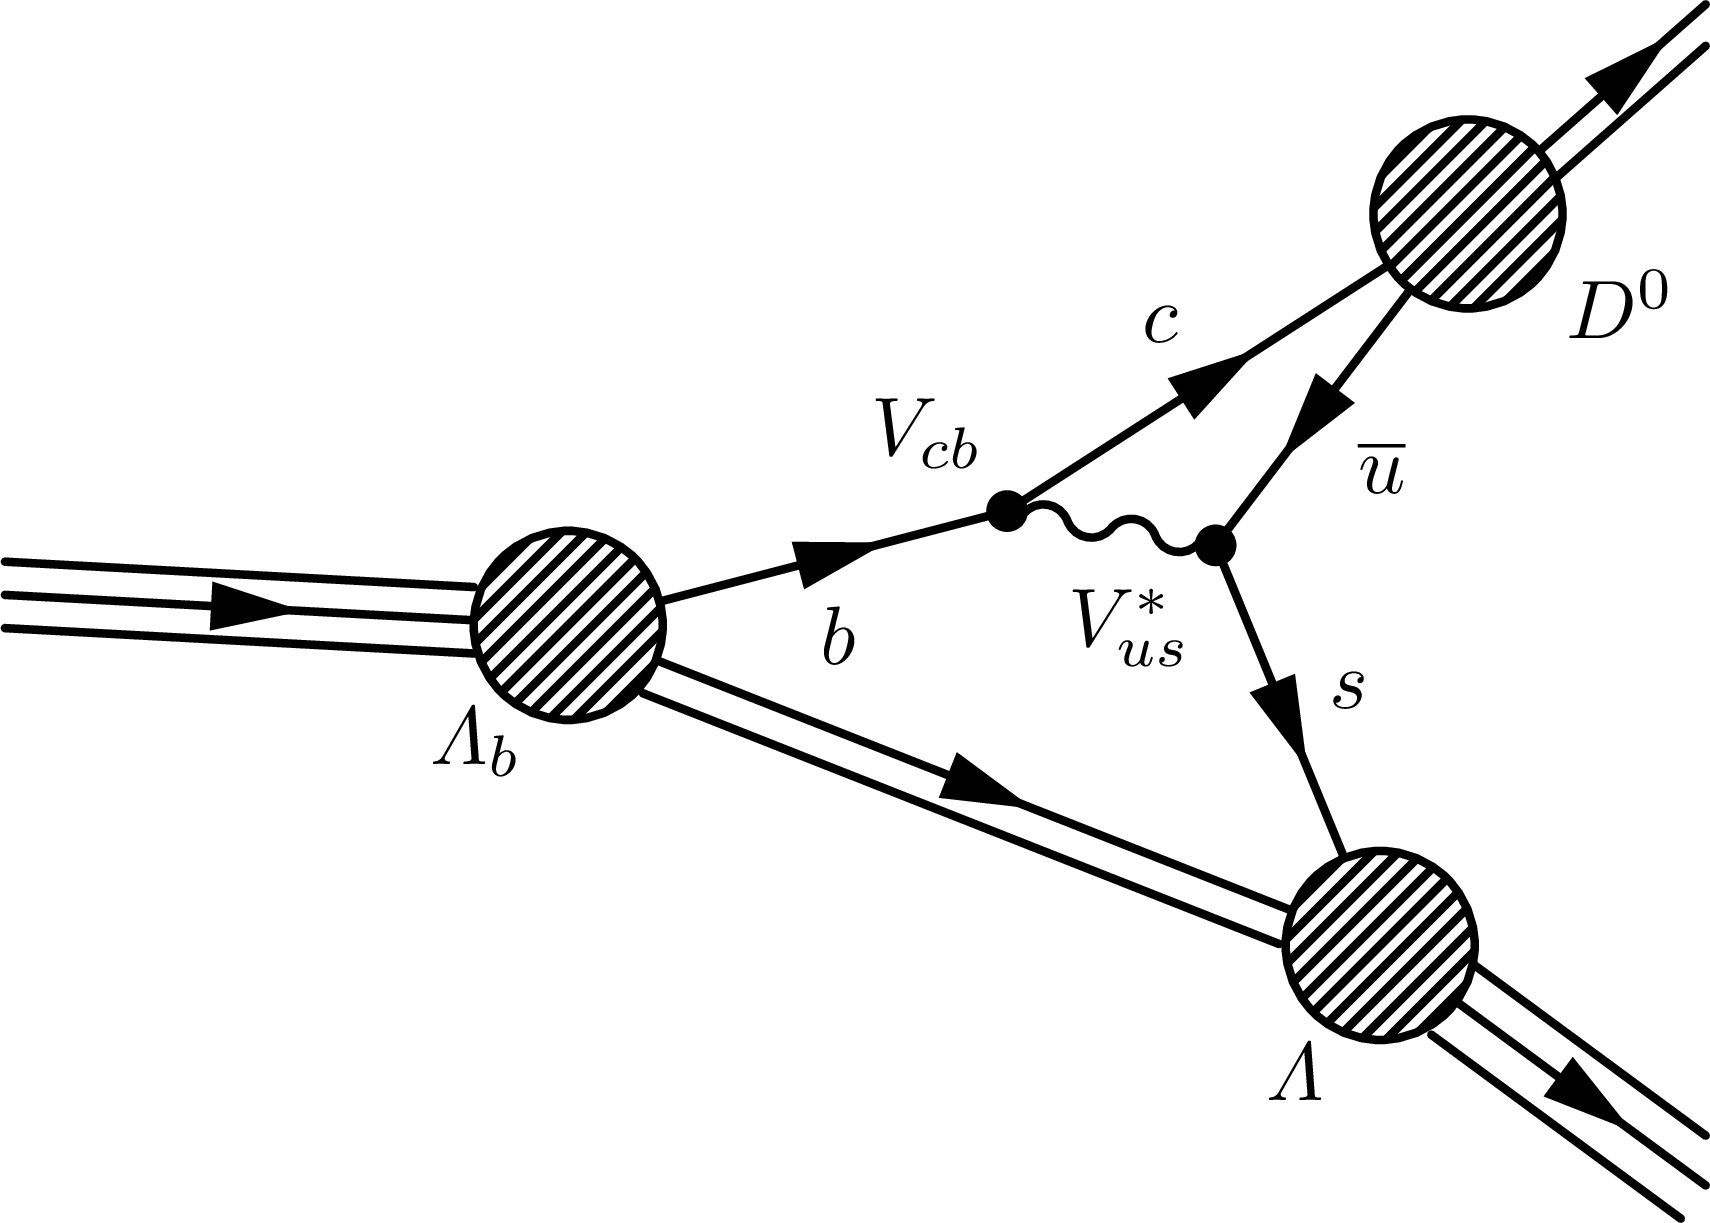
\includegraphics[height=.5\textheight]{misc/decayLb2DzLz}
        \end{column}
        \begin{column}{.45\textwidth}
            \centering
            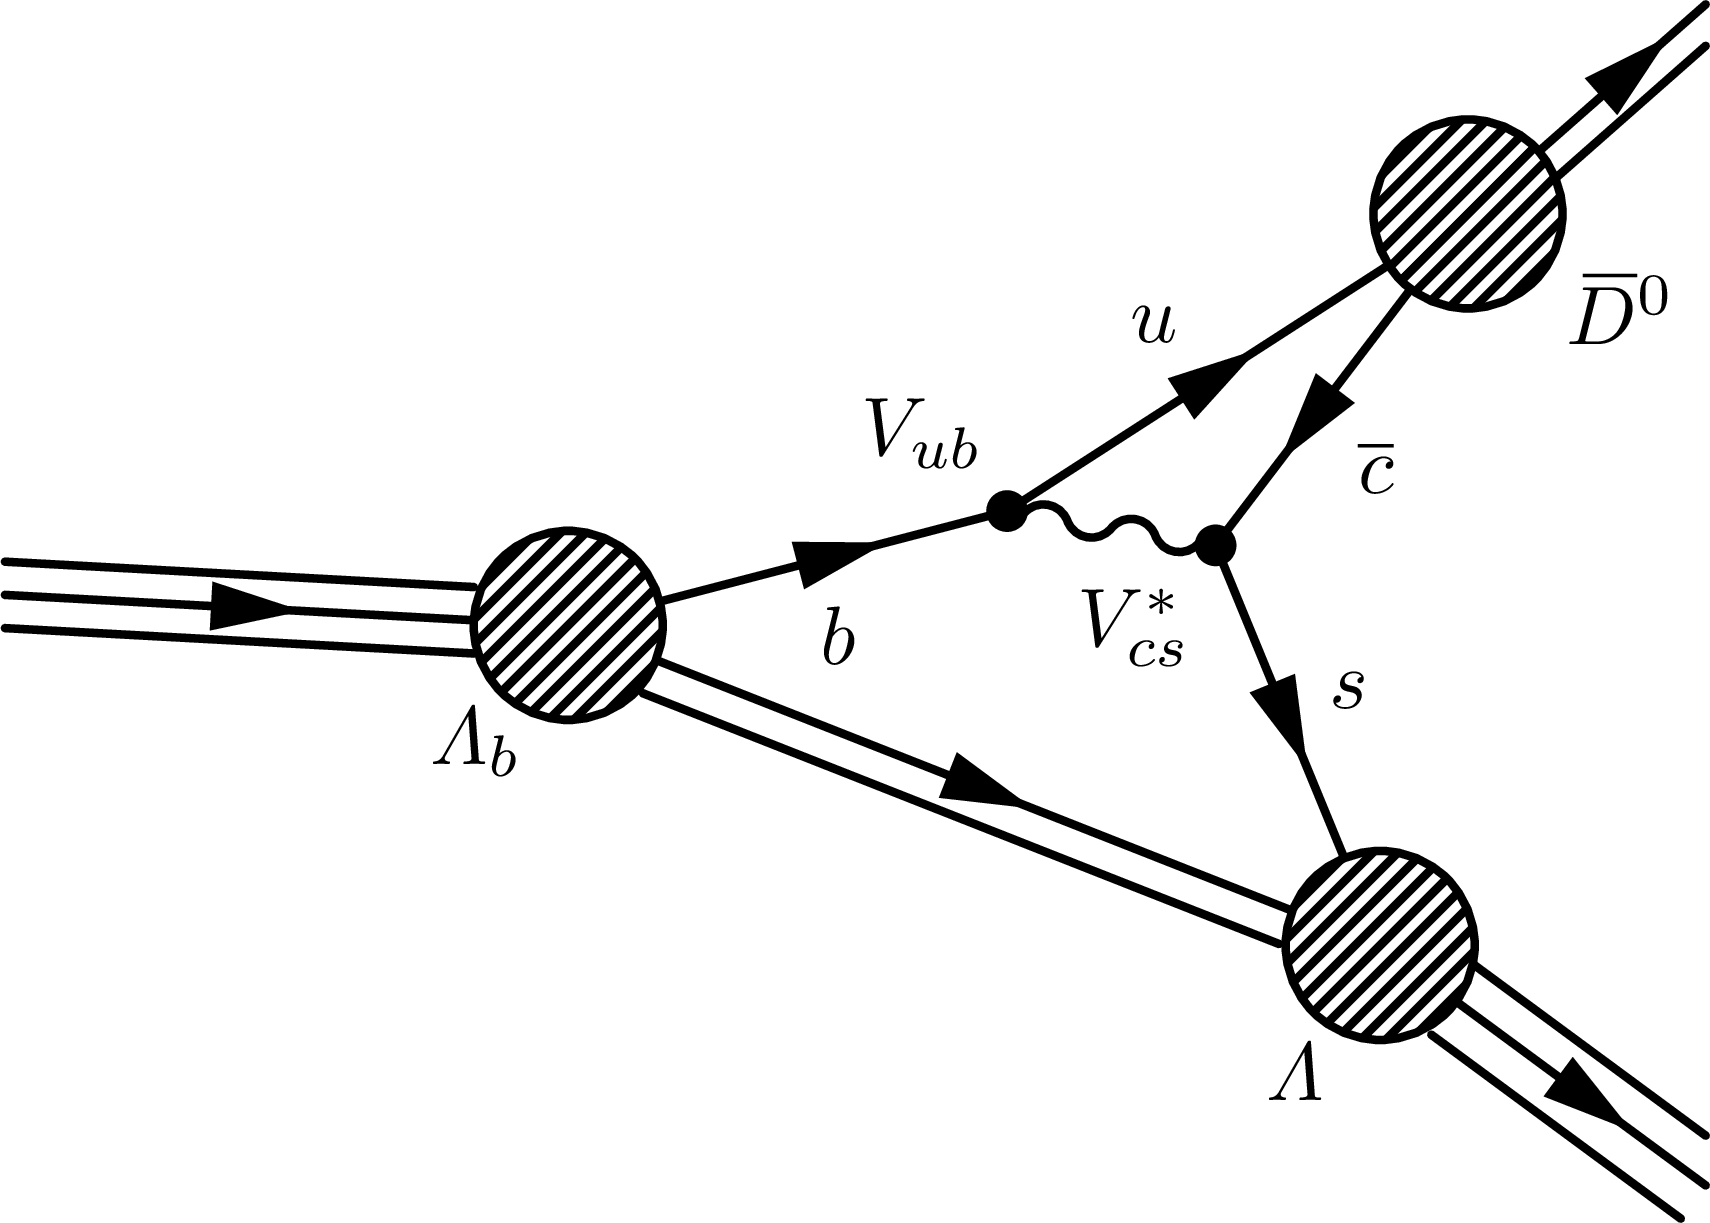
\includegraphics[height=.5\textheight]{misc/decayLb2DzbLz}
        \end{column}
    \end{columns}

    \begin{itemize}
        \item Perfectly suited for LHCb
        \item CKM angle: $\gamma + \mathcal{O}(\lambda^4)$ (without CPV in \Dz system)
        \item CPV in \decay{\Lb}{\Dz/\Dzb\Lz} and
        \begin{itemize}
            \item $\decay{\Dz/\Dzb}{\Kp\pim}$ (CPV but Cabibbo suppressed, \textbf{future prospect})
            \item $\decay{\Dz/\Dzb}{\Kp\Km \,/\, \pip\pim}$ (CPV but Cabibbo suppressed, \textbf{future prospect})
            \item $\decay{\Dz}{\Km\pip}$ (no CPV but Cabibbo favored, \textcolor{vertexDarkRed}{\textbf{this analysis}})
        \end{itemize}
    \end{itemize}
\end{frame}

\begin{frame}{Large Hadron Collider}
    \centering
    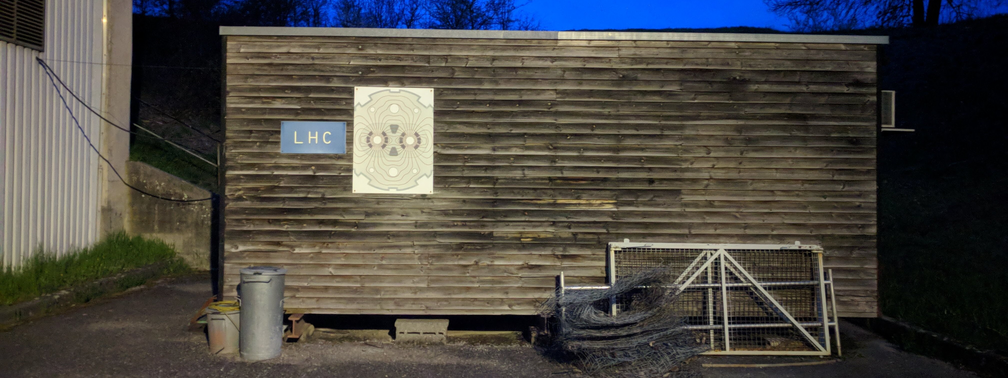
\includegraphics[height=.6\textheight]{lhc}\\
    \vspace{-2mm}
    \begin{center}
        \footnotesize (Symbolic image, picture taken at CERN site)
    \end{center}

    \begin{columns}[T]
        \begin{column}{.45\textwidth}
            \begin{itemize}
                \item World's largest and highest-energy particle accelerator 
                \item Built by CERN
            \end{itemize}
        \end{column}
        \begin{column}{.55\textwidth}
            \begin{itemize}
                \item Collides proton beams with $\sqrt{s}=13\,$TeV
                \item \bquark baryon factory (\Lb is lightest \bquark baryon)
            \end{itemize}
        \end{column}
    \end{columns}
\end{frame}

\begin{frame}{LHCb Experiment}
    \centering
    \enquote{LHCb is an experiment set up to explore what happened after the Big Bang that allowed matter to survive and build the Universe we inhabit today}

    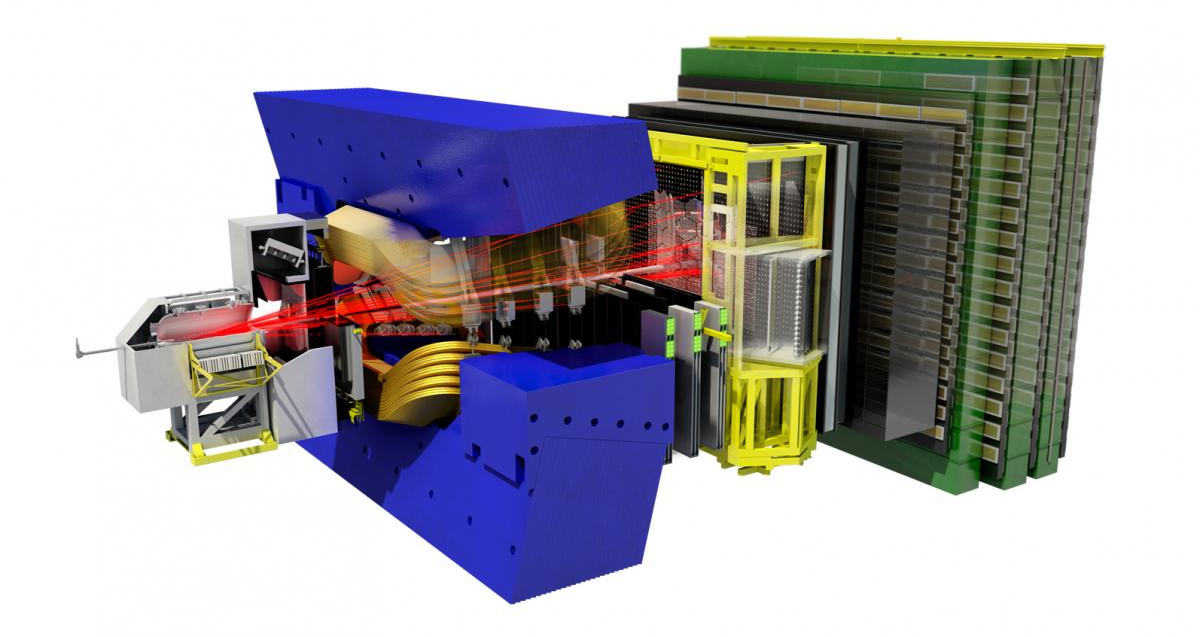
\includegraphics[height=.5\textheight]{detector}
    \begin{columns}[T]
        \begin{column}{.5\textwidth}
            \begin{itemize}
                \item One of the four major experiments at the LHC
                \item Dataset: $6\,\text{fb}^{-1}$ at $\sqrt{s}=13\,$TeV
            \end{itemize}
        \end{column}
        \begin{column}{.5\textwidth}
            \textbf{Multipurpose detector}, \eg{}:
            \begin{itemize}
                \item Excellent vertex resolution
                \item Powerful particle identification
            \end{itemize}
        \end{column}
    \end{columns}
\end{frame}

\begin{frame}{Outline}
    \scalebox{1.2}{\textbf{Why / What?}}
    \begin{itemize}
        \item Pave the way to measure CPV in decays of baryons at colliders
        \item Prose: search for the decays $$\decay{\Lb/\Xibz}{[\Km\pip]_{\Dz} \, [\proton\pim]_{\Lz}}$$
    \end{itemize}

    \scalebox{1.2}{\textbf{How?}}
    \begin{itemize}
        \item (Data calibration and pre-processing\ftntdagger)
        \item Classification of data as \textit{signal} and \textit{background} using MVA\ftntasterix
        \item (Study various physical backgrounds\ftntdagger)
        \item Count signal events with fit and estimate stat.\ significances\ftntasterix
        \item Estimate branching ratios $\mathcal{B}(\decay{\Lb}{\Dz\Lz})/\mathcal{B}(\decay{\Lb}{\Dz\proton\pim})$\ftntdagger{} and $\mathcal{B}(\decay{\Xibz}{\Dz\Lz})/\mathcal{B}(\decay{\Lb}{\Dz\Lz})$\ftntasterix
    \end{itemize}

    \footnotesize
    \ftntdagger not discussed here, \ftntasterix partially discussed here
\end{frame}
